\documentclass{standalone}
\usepackage{graphicx, standalone}
\usepackage[compat=1.1.0]{tikz-feynman}
\usepackage{tikz}
\usepackage{amsmath, amssymb}
\usepackage{euler}
\usepackage{fontspec}
\setmainfont{MinionPro}
\usepackage{comment}

\renewcommand{\k}{\ensuremath\text{k}}
\newcommand{\kp}{\ensuremath\text{k}'}
\newcommand{\q}{\ensuremath\text{q}}

\begin{document}

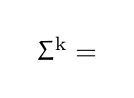
\begin{tikzpicture}[baseline=(current bounding box.center)]
	\node{$\Sigma^{\k}=$};
\end{tikzpicture}
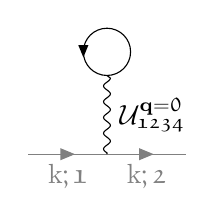
\begin{tikzpicture}[baseline=(current bounding box.base)]
	\begin{feynman}[small]
		\vertex (a);
		\vertex[right=of a] (b);
		\vertex[right=of b] (c);
		\vertex[above=of b] (b1);
		
		\vertex (u) at ($(b1)!0.5!(b)$);
		\node[right=0.1em of u] {$\mathcal{U}^{\textbf{q}=0}_{\mathfrak{1234}}$};
		
		\def\r{0.3}
		
		\path (b1)--++(90:\r) coordinate (A);
		\draw[fermion, arrow size=1pt] (A) circle(\r);		
		
		\diagram* {
			(a) -- [fermion, gray, edge label'=$\k;\mathfrak{1}$] (b) -- [fermion, gray, edge label'=$\k;\mathfrak{2}$] (c),
			(b) -- [photon] (b1)
		};	
	\end{feynman}
\end{tikzpicture}
\begin{tikzpicture}[baseline=(current bounding box.center)]
    \node {$+$};
\end{tikzpicture}
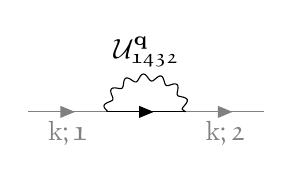
\begin{tikzpicture}[baseline=(current bounding box.base)]
	\begin{feynman}[small]
		\vertex (a);
		\vertex[right=of a] (b);
		\vertex[right=of b] (c);
		\vertex[right=of c] (d);
		\vertex (u) at ($(b)!0.5!(c)$);
		
		\node[above=0.45cm of u] {$\mathcal{U}^{\textbf{q}}_{\mathfrak{1432}}$};
		
		\diagram* {
			(a) -- [fermion, gray, edge label'=$\k;\mathfrak{1}$] (b),
			(b) -- [fermion] (c),
			(c) -- [fermion, gray, edge label'=$\k;\mathfrak{2}$] (d),
			(b) -- [photon, half left] (c)
		};
	\end{feynman}
\end{tikzpicture}
\begin{tikzpicture}[baseline=(current bounding box.center)]
    \node {$+$};
\end{tikzpicture}
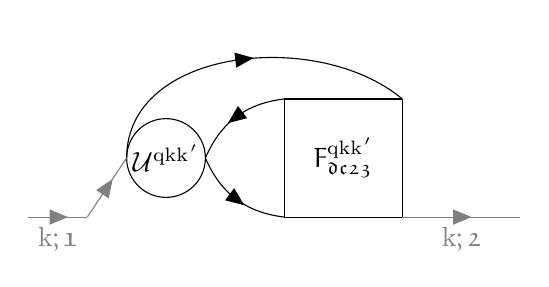
\begin{tikzpicture}[baseline=(current bounding box.base)]
	\begin{feynman}
		\vertex (a1);
		\vertex[right=0.75cm of a1] (a2);
		\vertex (b1) at ($(a2)+(0.5,0.75)$);
		\vertex[right=1cm of b1] (b3);
		\vertex (c2) at ($(b3)+(1,-0.75)$);
		\vertex[above=of c2] (c1);
		\vertex[right=of c1] (d1);
		\vertex[below=of d1] (d2);
		\vertex[right=of d2] (e1);
		
		\node (u) at ($(b1)!0.5!(b3)$) {$\mathcal{U}^{\q\k\kp}$};
		\draw (u) circle (0.5);

		\node at ($(c1)!0.5!(d2)$) {$F^{\q\k\kp}_{\mathfrak{dc23}}$};
		
		\diagram* {
			(a1) -- [fermion, gray, edge label'=$\k;\mathfrak{1}$] (a2) -- [fermion, gray] (b1),
			(d2) -- [fermion, gray, edge label'=$\k;\mathfrak{2}$] (e1),	
			(c1) -- (d1) -- (d2) -- (c2) -- (c1),	
			(c1) -- [fermion, bend right=30] (b3),
			(b3) -- [fermion, bend right=30] (c2),
			(b1) -- [fermion, in=140, out=90] (d1),
		};
	\end{feynman}
\end{tikzpicture}

\end{document}